
\chapter[Lý thuyết và bài tập: Cộng hưởng điện]{Lý thuyết và bài tập: Cộng hưởng điện}
\section{Lý thuyết}
\subsection{Điều kiện xảy ra hiện tượng cộng hưởng điện}

\begin{center}
	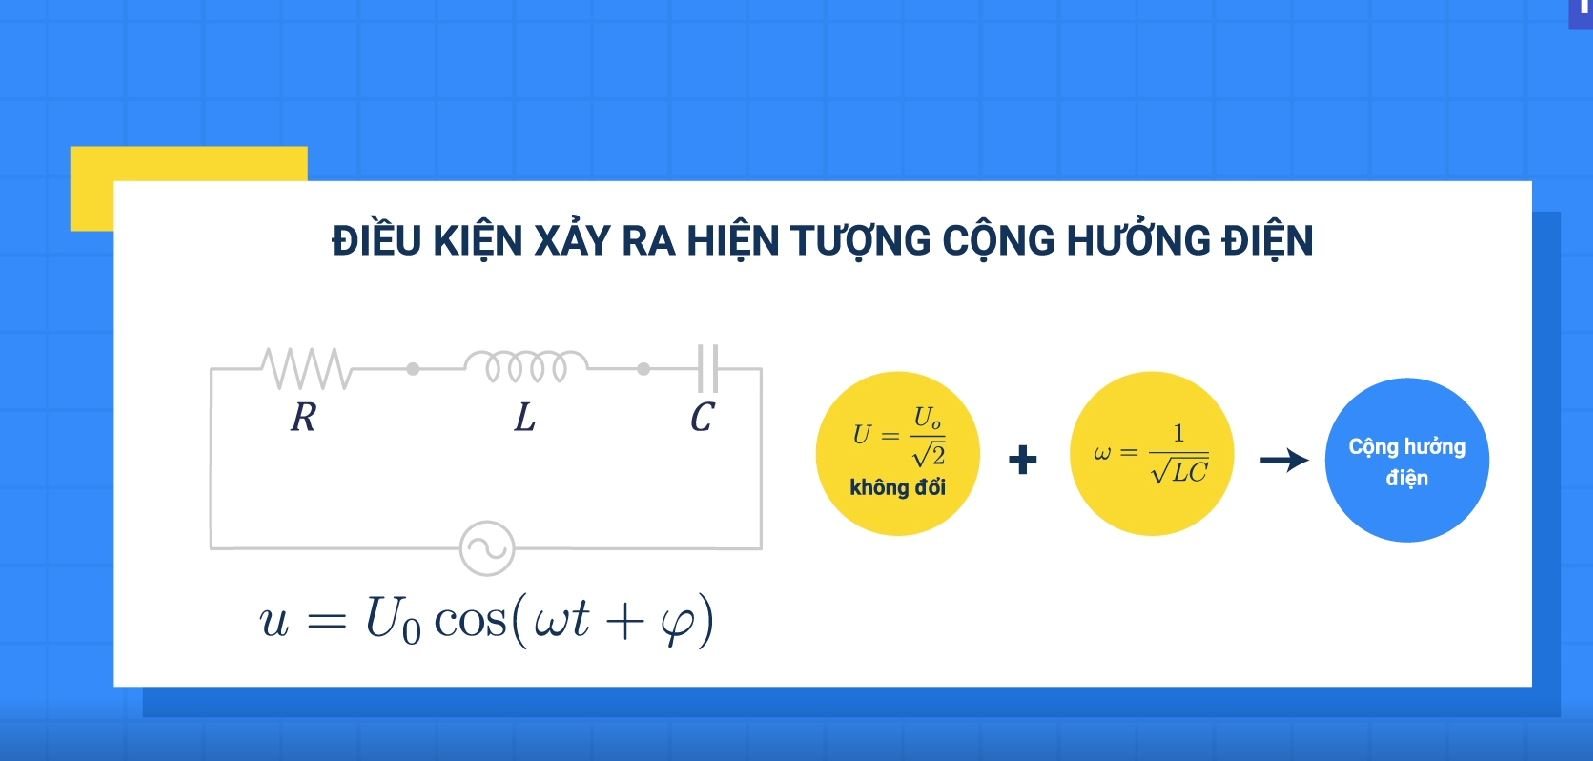
\includegraphics[scale=0.3]{../figs/VN12-PH-19-L-012-1-V2-2.jpg}
\end{center}

Cộng hưởng điện xảy ra khi
\begin{equation*}
	Z_L = Z_C,
\end{equation*}
hay
\begin{equation*}
	\omega ^2 LC =1.
\end{equation*}
Lúc đó tổng trở của mạch là $Z=R$, cường độ dòng điện hiệu dụng trong mạch có giá trị lớn nhất:
\begin{equation*}
	I=\dfrac{U}{R}.
\end{equation*}

\subsection{Đồ thị mô tả hiện tượng cộng hưởng điện}
Đồ thị mô tả sự phụ thuộc giữa công suất tiêu thụ toàn mạch vào tần số góc của dòng điện xoay chiều có dạng như sau:
\begin{center}
	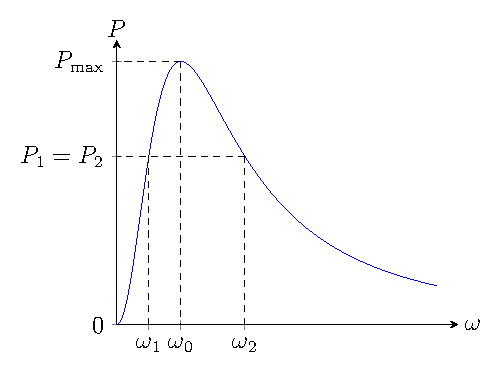
\includegraphics[scale=1,angle=0,clip=true,trim= 0mm 0 0 0]{../figs/VN12-PH-19-L-012-1-V2-1.pdf}
\end{center}
Trong đó $\omega_0=\dfrac{1}{\sqrt{LC}}$ là tần số góc của dòng điện khi xảy ra hiện tượng cộng hưởng điện.
\subsection{Một số dấu hiệu nhận biết hiện tượng cộng hưởng điện}

\begin{tabular}{|m{8em}|m{8em}|m{20em}|}
	\hline
	\thead{Đại lượng} & \thead{Công thức} & \multicolumn{1}{c|}{\thead{Mô tả}} \\ \hline
	\textbf{Tổng trở}    &  $$Z=R$$  & Tổng trở của mạch có giá trị nhỏ nhất và bằng $R$.                           \\ \hline
	\textbf{Cường độ dòng điện hiệu dụng} & $$I=\dfrac{U}{R}$$          &  Cường độ dòng điện hiệu dụng có giá trị lớn nhất.      \\ \hline
	\textbf{Điện áp hiệu dụng}                                                      &   $$U=U_R$$        &  Điện áp hiệu dụng giữa hai đầu đoạn mạch bằng điện áp hiệu dụng giữa hai đầu điện trở.                          \\ \hline
	\textbf{Công suất}                                                              &  $$P=UI=\dfrac{U^2}{R}$$   &  Công suất toàn mạch có giá trị lớn nhất và bằng công suất tiêu thụ trên điện trở.     \\ \hline
	\textbf{Hệ số công suất}                                                        &     $$\cos \varphi = 1$$      &  Hệ số công suất có giá trị lớn nhất.                          \\ \hline
	\textbf{Độ lệch pha}                                                            &   $$\varphi = \varphi_u - \varphi_i=0$$        &  Dòng điện cùng pha với điện áp.         \\ \hline
\end{tabular}
\section{Mục tiêu bài học - Ví dụ minh họa}
\begin{dang}{Nhận biết và giải thích được\\ hiện tượng cộng hưởng điện}
	\viduii{2}{Đặt điện áp $u=U_0 \cos \omega t$ ($U_0$ không đổi, $\omega$ thay đổi được) vào hai đầu đoạn mạch gồm điện trở $R$, cuộn cảm thuần có độ tự cảm $L$ và tụ điện có điện dung $C$ mắc nối tiếp. Hiện tượng cộng hưởng điện xảy ra khi
		\begin{mcq}(2)
			\item $\omega^2 LCR - 1 = 0$.
			\item $R=\left|\omega L - \dfrac{1}{\omega C}\right|$.
			\item $\omega^2 LC -1 =0$.
			\item $\omega^2 LC - R = 0$.
	\end{mcq}}	
	{\begin{center}
			\textbf{Hướng dẫn giải}
		\end{center}
		Khi xảy ra hiện tượng cộng hưởng điện:
		\begin{equation*}
			Z_L = Z_C \Leftrightarrow \omega L =\dfrac{1}{\omega C} \Leftrightarrow \omega ^2 = \dfrac{1}{LC} \Leftrightarrow \omega^2 LC -1 =0.
		\end{equation*}
		
		\textbf{Đáp án: C.}
		
	}
	\viduii{2}{Cho đoạn mạch điện xoay chiều gồm cuộn dây thuần cảm $L$, tụ điện $C$ và biến trở $R$ mắc nối tiếp. Khi đặt vào hai đầu mạch một điện áp xoay chiều ổn định có tần số $f$ thì thấy $4\pi^2f^2LC = 1$. Khi thay đổi R thì
		\begin{mcq}
			\item điện áp hiệu dụng giữa hai đầu biến trở thay đổi.
			\item tổng trở của mạch vẫn không đổi.
			\item công suất tiêu thụ trên mạch thay đổi.
			\item hệ số công suất trên mạch thay đổi.
	\end{mcq}}	
	{\begin{center}
			\textbf{Hướng dẫn giải}
		\end{center}
		Từ điều kiện $4\pi^2f^2LC = 1$ suy ra $Z_L = Z_C$, tức là trong mạch xảy ra cộng hưởng và lúc này:
		
		$$U_R = U \text{ với mọi } R$$
		
		Mà:
		$$Z= \sqrt {R^2 + (Z_L - Z_C)^2} =R \Rightarrow Z\ \text{thay đổi}.$$
		
		$$P = \dfrac{U^2}{R} \Rightarrow P\ \text{thay đổi}.$$
		
		$$\cos \varphi = \dfrac{R}{Z} =1 \text{ với mọi } R$$
		
		
		
		\textbf{Đáp án: C.}
		
	}
\end{dang}
\begin{dang}{Ứng dụng điều kiện xảy ra hiện tượng cộng hưởng để xác định các đại lượng trong dòng điện xoay chiều}
	\viduii{2}{Đặt điện áp xoay chiều $u=U \sqrt 2 \cos 100 \pi t\ \text{(V)}$ ($t$ tính bằng $\SI{}{\second}$) vào hai đầu đoạn mạch có $R$, $L$, $C$ mắc nối tiếp thì có cộng hưởng điện. Biết cuộn cảm có cảm kháng $\SI{80}{\Omega}$. Điện dung của tụ điện có giá trị là
		\begin{mcq}(2)
			\item $\SI{0.25}{\farad}$.
			\item $\SI{1.25e-4}{\farad}$.
			\item $\SI{3.98e-5}{\farad}$.
			\item $\SI{0.80}{\farad}$.
	\end{mcq}}	
	{\begin{center}
			\textbf{Hướng dẫn giải}
		\end{center}
		Khi xảy ra hiện tượng cộng hưởng điện:
		\begin{equation*}
			Z_L = Z_C \Leftrightarrow Z_L = \dfrac{1}{\omega C} \Leftrightarrow C  = \dfrac{1}{\omega Z_L} \approx \SI{3.98e-5}{\farad}.
		\end{equation*}
		
		\textbf{Đáp án: C.}
		
	}
	\viduii{2}{Đặt điện áp xoay chiều $u=60\sqrt 2 \cos 100 \pi t \ \text{(V)}$ ($t$ tính bằng $\SI{}{\second}$) vào hai đầu đoạn mạch mắc nối tiếp gồm điện trở $\SI{30}{\Omega}$, tụ điện có điện dung $\dfrac{10^{-3}}{4\pi}\ \text F$ và cuộn cảm thuần có độ tự cảm $L$ thay đổi được. Điều chỉnh $L$ để cường độ hiệu dụng của dòng điện trong mạch đạt cực đại. Khi đó, điện áp hiệu dụng giữa hai đầu cuộn cảm là
		\begin{mcq}(4)
			\item $\SI{80}{\volt}$.
			\item $80\sqrt2\ \text V$.
			\item $60\sqrt2\ \text V$.
			\item $60\ \text V$.
	\end{mcq}}
	{\begin{center}
			\textbf{Hướng dẫn giải}
		\end{center}
		Khi xảy ra hiện tượng cộng hưởng điện, cường độ dòng điện hiệu dụng trong mạch đạt cực đại:
		\begin{equation*}
			I=\dfrac{U}{R}=\SI{2}{\ampere}.
		\end{equation*}
		
		Ngoài ra, cảm kháng $Z_L$ bằng dung kháng $Z_C$, suy ra \begin{equation*}
			Z_L=Z_C=\dfrac{1}{\omega C} = \SI{40}{\Omega}.
		\end{equation*}
		
		Điện áp hiệu dụng giữa hai đầu cuộn cảm:
		\begin{equation*}
			U_L = I Z_L = \SI{80}{\volt}.
		\end{equation*}
		
		\textbf{Đáp án: A.}
	}
\end{dang}